\documentclass{article}

\usepackage{pandekten}
\usepackage{dashrule}

\makeatletter
\newcommand*{\shifttext}[1]{%
  \settowidth{\@tempdima}{#1}%
  \hspace{-\@tempdima}#1%
}
\newcommand{\plabel}[1]{%
\shifttext{\textbf{#1}\quad}%
}
\newcommand{\prule}{%
\begin{center}%
\hdashrule[0.5ex]{.99\linewidth}{1pt}{1pt 2.5pt}%
\end{center}%
}

\makeatother

\newcommand{\minusbaseline}{\abovedisplayskip=0pt\abovedisplayshortskip=0pt~\vspace*{-\baselineskip}}%

\setlength{\parindent}{0pt}

\title{Assignment 9}
\author{Ze Chen}

\begin{document}

\maketitle

\plabel{1 (a)}%
For $\lambda = 0$,
\[ H = \int \dd[3]{x} \sum_i \qty(\frac{1}{2} (\Pi^i)^2 + \frac{1}{2} (\grad \Phi^i)^2 + \frac{1}{2} m^2 (\Phi^i)^2), \]
which consists of $N$ independent real scalar fields, and therefore the propagators are just
\[ \wick{\c1 \Phi^i(x) \c1 \Phi^j(y)} = \delta^{ij} D_{\mathrm{F}}(x-y). \]
The vertex is given by
\begin{align*}
  &\phantom{{}={}} 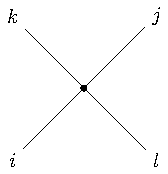
\includegraphics{img/phi4/phi4.pdf} \\
  &= -i\frac{\lambda}{4} \sum_p \sum_q \text{number of contractions of } \qty(\Phi^i \Phi^j \Phi^k \Phi^l \Phi^p \Phi^p \Phi^q \Phi^q) \\
  &= -i \frac{\lambda}{4} \sum_p \sum_q 4\big(
    \delta^{ip}\delta^{jp}\delta^{kq}\delta^{lq} + \delta^{ip}\delta^{kp}\delta^{jq}\delta^{lq} + \delta^{ip}\delta^{lp}\delta^{jq}\delta^{kq}\\
  &\phantom{-i \frac{\lambda}{4} \sum_p \sum_q 4\big(} + \delta^{jp}\delta^{kp}\delta^{iq}\delta^{lq} + \delta^{jp}\delta^{lp}\delta^{iq}\delta^{kq} + + \delta^{kp}\delta^{lp}\delta^{iq}\delta^{jq}\big) \\
  &= -2 i \lambda\qty(\delta^{ij}\delta^{kl} + \delta^{il}\delta^{jk} + \delta^{ik} \delta^{jl}).
\end{align*}
The differential cross section is given by
\[ \qty(\dv{\sigma}{\Omega})_{\mathrm{CM}} = \frac{\abs{\mathcal{M}}^2}{64\pi^2 E^2_{\mathrm{cm}}} \]
where
\begin{align*}
  \abs{\mathcal{M}(\Phi^1\Phi^2 \rightarrow \Phi^1\Phi^2)}^2 &= 4\lambda^2, \\
  \abs{\mathcal{M}(\Phi^1\Phi^1 \rightarrow \Phi^2\Phi^2)}^2 &= 4\lambda^2, \\
  \abs{\mathcal{M}(\Phi^1\Phi^1 \rightarrow \Phi^1\Phi^1)}^2 &= 36\lambda^2.
\end{align*}

\end{document}
